% Options for packages loaded elsewhere
\PassOptionsToPackage{unicode}{hyperref}
\PassOptionsToPackage{hyphens}{url}
\PassOptionsToPackage{dvipsnames,svgnames,x11names}{xcolor}
\documentclass[
  11pt,
  fontset=fandol]{ctexart}
\usepackage{xcolor}
\usepackage{amsmath,amssymb}
\setcounter{secnumdepth}{-\maxdimen} % remove section numbering
\usepackage{iftex}
\ifPDFTeX
  \usepackage[T1]{fontenc}
  \usepackage[utf8]{inputenc}
  \usepackage{textcomp} % provide euro and other symbols
\else % if luatex or xetex
  \usepackage{unicode-math} % this also loads fontspec
  \defaultfontfeatures{Scale=MatchLowercase}
  \defaultfontfeatures[\rmfamily]{Ligatures=TeX,Scale=1}
\fi
\usepackage{lmodern}
\ifPDFTeX\else
  % xetex/luatex font selection
    \setmainfont[BoldFont=texgyrepagella-bold.otf,ItalicFont=texgyrepagella-italic.otf,BoldItalicFont=texgyrepagella-bolditalic.otf]{texgyrepagella-regular.otf}
    \setsansfont[BoldFont=texgyreheros-bold.otf,ItalicFont=texgyreheros-italic.otf,BoldItalicFont=texgyreheros-bolditalic.otf]{texgyreheros-regular.otf}
    \setmonofont[]{lmmono10-regular.otf}
\fi
% Use upquote if available, for straight quotes in verbatim environments
\IfFileExists{upquote.sty}{\usepackage{upquote}}{}
\IfFileExists{microtype.sty}{% use microtype if available
  \usepackage[]{microtype}
  \UseMicrotypeSet[protrusion]{basicmath} % disable protrusion for tt fonts
}{}
\makeatletter
\@ifundefined{KOMAClassName}{% if non-KOMA class
  \IfFileExists{parskip.sty}{%
    \usepackage{parskip}
  }{% else
    \setlength{\parindent}{0pt}
    \setlength{\parskip}{6pt plus 2pt minus 1pt}}
}{% if KOMA class
  \KOMAoptions{parskip=half}}
\makeatother
\usepackage{color}
\usepackage{fancyvrb}
\newcommand{\VerbBar}{|}
\newcommand{\VERB}{\Verb[commandchars=\\\{\}]}
\DefineVerbatimEnvironment{Highlighting}{Verbatim}{commandchars=\\\{\}}
% Add ',fontsize=\small' for more characters per line
\newenvironment{Shaded}{}{}
\newcommand{\AlertTok}[1]{\textcolor[rgb]{1.00,0.00,0.00}{\textbf{#1}}}
\newcommand{\AnnotationTok}[1]{\textcolor[rgb]{0.38,0.63,0.69}{\textbf{\textit{#1}}}}
\newcommand{\AttributeTok}[1]{\textcolor[rgb]{0.49,0.56,0.16}{#1}}
\newcommand{\BaseNTok}[1]{\textcolor[rgb]{0.25,0.63,0.44}{#1}}
\newcommand{\BuiltInTok}[1]{\textcolor[rgb]{0.00,0.50,0.00}{#1}}
\newcommand{\CharTok}[1]{\textcolor[rgb]{0.25,0.44,0.63}{#1}}
\newcommand{\CommentTok}[1]{\textcolor[rgb]{0.38,0.63,0.69}{\textit{#1}}}
\newcommand{\CommentVarTok}[1]{\textcolor[rgb]{0.38,0.63,0.69}{\textbf{\textit{#1}}}}
\newcommand{\ConstantTok}[1]{\textcolor[rgb]{0.53,0.00,0.00}{#1}}
\newcommand{\ControlFlowTok}[1]{\textcolor[rgb]{0.00,0.44,0.13}{\textbf{#1}}}
\newcommand{\DataTypeTok}[1]{\textcolor[rgb]{0.56,0.13,0.00}{#1}}
\newcommand{\DecValTok}[1]{\textcolor[rgb]{0.25,0.63,0.44}{#1}}
\newcommand{\DocumentationTok}[1]{\textcolor[rgb]{0.73,0.13,0.13}{\textit{#1}}}
\newcommand{\ErrorTok}[1]{\textcolor[rgb]{1.00,0.00,0.00}{\textbf{#1}}}
\newcommand{\ExtensionTok}[1]{#1}
\newcommand{\FloatTok}[1]{\textcolor[rgb]{0.25,0.63,0.44}{#1}}
\newcommand{\FunctionTok}[1]{\textcolor[rgb]{0.02,0.16,0.49}{#1}}
\newcommand{\ImportTok}[1]{\textcolor[rgb]{0.00,0.50,0.00}{\textbf{#1}}}
\newcommand{\InformationTok}[1]{\textcolor[rgb]{0.38,0.63,0.69}{\textbf{\textit{#1}}}}
\newcommand{\KeywordTok}[1]{\textcolor[rgb]{0.00,0.44,0.13}{\textbf{#1}}}
\newcommand{\NormalTok}[1]{#1}
\newcommand{\OperatorTok}[1]{\textcolor[rgb]{0.40,0.40,0.40}{#1}}
\newcommand{\OtherTok}[1]{\textcolor[rgb]{0.00,0.44,0.13}{#1}}
\newcommand{\PreprocessorTok}[1]{\textcolor[rgb]{0.74,0.48,0.00}{#1}}
\newcommand{\RegionMarkerTok}[1]{#1}
\newcommand{\SpecialCharTok}[1]{\textcolor[rgb]{0.25,0.44,0.63}{#1}}
\newcommand{\SpecialStringTok}[1]{\textcolor[rgb]{0.73,0.40,0.53}{#1}}
\newcommand{\StringTok}[1]{\textcolor[rgb]{0.25,0.44,0.63}{#1}}
\newcommand{\VariableTok}[1]{\textcolor[rgb]{0.10,0.09,0.49}{#1}}
\newcommand{\VerbatimStringTok}[1]{\textcolor[rgb]{0.25,0.44,0.63}{#1}}
\newcommand{\WarningTok}[1]{\textcolor[rgb]{0.38,0.63,0.69}{\textbf{\textit{#1}}}}
\usepackage{longtable,booktabs,array}
\usepackage{calc} % for calculating minipage widths
% Correct order of tables after \paragraph or \subparagraph
\usepackage{etoolbox}
\makeatletter
\patchcmd\longtable{\par}{\if@noskipsec\mbox{}\fi\par}{}{}
\makeatother
% Allow footnotes in longtable head/foot
\IfFileExists{footnotehyper.sty}{\usepackage{footnotehyper}}{\usepackage{footnote}}
\makesavenoteenv{longtable}
\usepackage{graphicx}
\makeatletter
\newsavebox\pandoc@box
\newcommand*\pandocbounded[1]{% scales image to fit in text height/width
  \sbox\pandoc@box{#1}%
  \Gscale@div\@tempa{\textheight}{\dimexpr\ht\pandoc@box+\dp\pandoc@box\relax}%
  \Gscale@div\@tempb{\linewidth}{\wd\pandoc@box}%
  \ifdim\@tempb\p@<\@tempa\p@\let\@tempa\@tempb\fi% select the smaller of both
  \ifdim\@tempa\p@<\p@\scalebox{\@tempa}{\usebox\pandoc@box}%
  \else\usebox{\pandoc@box}%
  \fi%
}
% Set default figure placement to htbp
\def\fps@figure{htbp}
\makeatother
\setlength{\emergencystretch}{3em} % prevent overfull lines
\providecommand{\tightlist}{%
  \setlength{\itemsep}{0pt}\setlength{\parskip}{0pt}}
% Portable CJK typography: ctex + the open Fandol font family.
\usepackage{geometry}
\geometry{a4paper,left=24mm,right=24mm,top=25mm,bottom=25mm,headheight=15pt}
\usepackage{xcolor}
\definecolor{inkblue}{HTML}{254B62}
\definecolor{muted}{HTML}{657681}
\usepackage{setspace}
\setstretch{1.42}
\setlength{\parindent}{2em}
\setlength{\parskip}{0.28em}
\setlength{\emergencystretch}{3em}
\ctexset{
  section={format=\Large\sffamily\bfseries\color{inkblue},beforeskip=1.7em,afterskip=.8em},
  subsection={format=\large\sffamily\bfseries\color{inkblue},beforeskip=1.3em,afterskip=.6em}
}
\usepackage{fancyhdr}
\providecommand{\LectureRunningTitle}{课程讲义}
\providecommand{\LectureCourseLabel}{南京大学 · 生成式软件工程}
\pagestyle{fancy}
\fancyhf{}
\fancyhead[L]{\small\sffamily\color{muted}\LectureRunningTitle}
\fancyhead[R]{\small\sffamily\color{muted}课程讲义}
\fancyfoot[C]{\small\color{muted}\thepage}
\renewcommand{\headrulewidth}{0.3pt}
\renewcommand{\footrulewidth}{0pt}
\usepackage{titling}
\pretitle{\begin{center}\LARGE\sffamily\bfseries\color{inkblue}}
\posttitle{\par\end{center}\vskip .8em}
\predate{\begin{center}}
\postdate{\end{center}}
\setlength{\droptitle}{-2em}
\renewcommand{\maketitle}{%
  \begin{center}
  {\LARGE\sffamily\bfseries\color{inkblue}\thetitle\par}
  \vspace{5mm}
  {\small\sffamily\color{muted}\LectureCourseLabel}
  \end{center}\vspace{4mm}\thispagestyle{fancy}}
\usepackage{needspace}
\usepackage{fvextra}
\DefineVerbatimEnvironment{Highlighting}{Verbatim}{breaklines,commandchars=\\\{\},fontsize=\small,frame=single,rulecolor=\color{muted},framesep=8pt}
\AtBeginDocument{\hypersetup{colorlinks=true,linkcolor=inkblue,urlcolor=inkblue,bookmarksopen=true}}
\AtBeginDocument{\urlstyle{same}}
\widowpenalty=10000
\clubpenalty=10000
\usepackage{bookmark}
\IfFileExists{xurl.sty}{\usepackage{xurl}}{} % add URL line breaks if available
\urlstyle{same}
\hypersetup{
  pdftitle={提示词与上下文工程：把要求、证据与探索组织起来},
  colorlinks=true,
  linkcolor={Maroon},
  filecolor={Maroon},
  citecolor={Blue},
  urlcolor={Blue},
  pdfcreator={LaTeX via pandoc}}

\title{提示词与上下文工程：把要求、证据与探索组织起来}
\author{}
\date{}

\renewcommand{\LectureRunningTitle}{提示词与上下文工程 · 南京大学 GSE 2026}
\renewcommand{\LectureCourseLabel}{南京大学 · 生成式软件工程 · 第 2 讲}
\begin{document}
\maketitle

课程：南京大学《生成式软件工程》2026 年第 2 讲；主讲：蒋炎岩。

视频：\href{https://www.bilibili.com/video/BV1CQt365EzW/}{《提示词工程》课程回放}，页面时长
1:38:26。

本文按问题重组课程内容，结合完整原视频、本地音轨转录、选定课堂画面及\href{https://jyywiki.cn/GSE/2026/lect2.md}{官方讲义}。转录时间采用真实的
20 秒输入窗口，不是逐字对齐；配图时间标示候选帧所在的 30
秒区间。正文中的编辑练习与参考资料补充均单独说明。主题与画面核验不代表逐字听写、逐帧审查或复现全部演示。

\section{学习目标}\label{ux5b66ux4e60ux76eeux6807}

读完本讲，应能解释为什么一句提示词不足以决定 Agent
的行为，怎样把模糊愿望改写为可检查的要求，怎样复用做事方法，以及为什么长程研究和开放探索需要比``多花
token''更具体的反馈与筛选机制。

\section{1.
提示词为什么不只在对话框里}\label{ux63d0ux793aux8bcdux4e3aux4ec0ux4e48ux4e0dux53eaux5728ux5bf9ux8bddux6846ux91cc}

聊天界面使人习惯把 prompt 理解成最后发出去的一句话。但 Agent
作决定时，看到的是一份已经组织起来的上下文：外围运行系统的指令、工具定义、项目文件、历史消息、加载的技能，以及本轮任务的要求。外围系统常被称为
harness，负责把模型接入工具和执行环境。

可以用条件概率 \(\Pr(\text{token}\mid\text{context})\)
描述下一步生成的基本视角。这里的 context
并不是``用户最后一句话''的同义词；已有代码怎样写，前面做过什么，刚刚返回了怎样的测试结果，都可能改变后续行为。

\Needspace{11\baselineskip}

\begin{longtable}[]{@{}
  >{\raggedright\arraybackslash}p{(\linewidth - 4\tabcolsep) * \real{0.3333}}
  >{\raggedright\arraybackslash}p{(\linewidth - 4\tabcolsep) * \real{0.3333}}
  >{\raggedright\arraybackslash}p{(\linewidth - 4\tabcolsep) * \real{0.3333}}@{}}
\toprule\noalign{}
\begin{minipage}[b]{\linewidth}\raggedright
上下文材料
\end{minipage} & \begin{minipage}[b]{\linewidth}\raggedright
主要作用
\end{minipage} & \begin{minipage}[b]{\linewidth}\raggedright
需要分清的边界
\end{minipage} \\
\midrule\noalign{}
\endhead
\bottomrule\noalign{}
\endlastfoot
系统和工具规则 & 约定运行与操作方式 & 具体来源和优先级由运行环境决定 \\
项目约定与 skill & 保存本项目惯例和任务方法 &
适用范围应清楚，避免无关规则堆积 \\
用户目标与反馈 & 指定当前任务和取舍 & 新反馈可能修正原来的目标 \\
代码、文档、工具输出 & 提供事实、状态、样例与证据 &
被读取的材料不自动拥有下命令的资格 \\
\end{longtable}

因此，上下文工程关心的是：在关键决定发生时，模型能看见哪些信息，这些信息分别承担什么作用。增加文字只是一个手段；删去过时记录、提供现有实现、把验证结果放在合适的位置，同样是在组织上下文。

\par\addvspace{1em}\noindent\begin{minipage}{\linewidth}\centering


\includegraphics[width=0.94\linewidth,height=8.5cm,keepaspectratio]{notes/pce_context.jpg}

\textbf{上下文组成与条件生成}

\raggedright\footnotesize\color{muted}

画面证据：原视频
02:30--03:00，\href{https://www.bilibili.com/video/BV1CQt365EzW/?t=150}{回看课堂片段}。课堂列出系统、项目、技能、工具与历史材料，并区分内容与指令。

\end{minipage}\par\addvspace{1em}

\subsection{``安全命令''为什么不能只靠一句话判断}\label{ux5b89ux5168ux547dux4ee4ux4e3aux4ec0ux4e48ux4e0dux80fdux53eaux9760ux4e00ux53e5ux8bddux5224ux65ad}

课堂讨论了 Agent 执行命令时的权限与审批。模型会提出动作，harness
可能依据规则决定是否询问，操作系统再落实实际的访问限制。这几个环节不能混在一起：模型愿意遵守要求，不等于程序已经实现了可靠的权限边界。

让 Agent
说明它在当前任务中有哪些可公开的目标、工具规则和项目约定，可以帮助使用者理解工作方式；模型自述仍不是实现机制的完整证明。判断某次行为为什么发生，应结合可访问的配置、源码、操作记录和结果，不应要求或假定能读取隐藏的内部指令。

课堂的具体做法，是从``为什么有些命令要确认，有些不用''出发，让 Agent
阅读当时下载的实现，追踪静态规则、风险判定和审批路径，并讨论修改后观察行为的办法。这个例子的重点是从现象追到机制、再寻找证据；不能把现场某次回答直接推广为所有版本的产品事实。

\par\addvspace{1em}\noindent\begin{minipage}{\linewidth}\centering

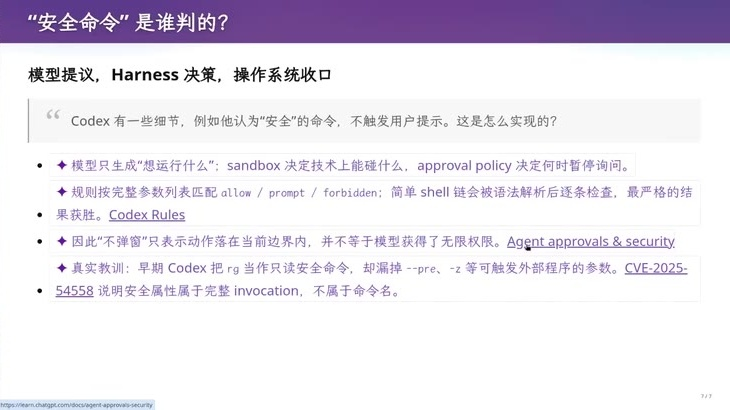
\includegraphics[width=0.94\linewidth,height=8.5cm,keepaspectratio]{notes/pce_safety.jpg}

\textbf{模型、外围系统与操作系统的分工}

\raggedright\footnotesize\color{muted}

画面证据：原视频
12:30--13:00，\href{https://www.bilibili.com/video/BV1CQt365EzW/?t=750}{回看课堂片段}。用于说明课堂如何拆分执行机制，不作为当前所有产品版本行为的独立验证。

\end{minipage}\par\addvspace{1em}

\section{2. AI
降低的是开始行动的门槛}\label{ai-ux964dux4f4eux7684ux662fux5f00ux59cbux884cux52a8ux7684ux95e8ux69db}

课堂把 AI
描述成一个耐心的学习伙伴。一个推导不愿意验算，一条数据通路始终没弄懂，或者不知道链接阶段做了什么，过去可能因为搜索和试错成本太高而长期搁置。现在可以立即要求一个最小例子、一次推导或一段可运行程序，再围绕结果继续追问。

这种便利并不自动等于学会。读答案时觉得顺畅，与自己能够解释，是两种不同的状态。更有用的循环是：先提出具体问题，借助资料理解，再离开原答案用自己的话重述；把讲不清的地方交给听众追问，最后回到推导、原文或实验核对。

课堂的``让 AI
当听众''强调主动组织知识。它可以提出反例和问题，替你指出解释中的跳步；最后能否重新说清楚，仍然要由学习者自己完成。开场关于
token
和退学的夸张说法，是在推动立即实践，不能当成真实退学要求或消费建议。

本章小结：把``以后再学''改成一个现在就能验证的小问题，比收集更多看起来完整的答案更有价值。

\par\addvspace{1em}\noindent\begin{minipage}{\linewidth}\centering

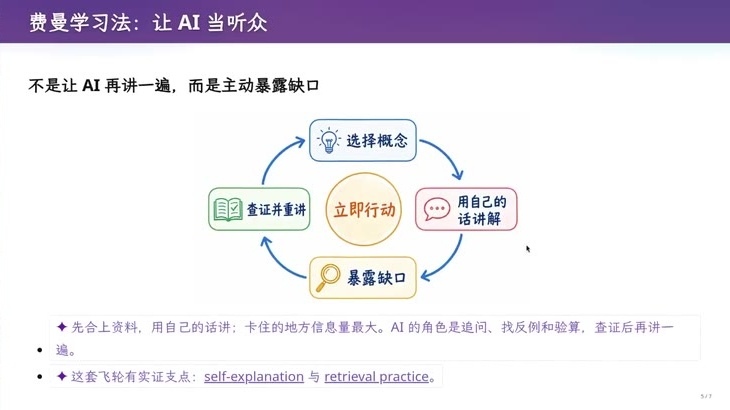
\includegraphics[width=0.94\linewidth,height=8.5cm,keepaspectratio]{notes/pce_learning.jpg}

\textbf{用复述与追问暴露理解缺口}

\raggedright\footnotesize\color{muted}

画面证据：原视频
10:00--10:30，\href{https://www.bilibili.com/video/BV1CQt365EzW/?t=600}{回看课堂片段}。课堂把学习组织为选择概念、自己解释、暴露缺口与查证重讲的循环。

\end{minipage}\par\addvspace{1em}

\section{3.
怎样让模型知道什么才算完成}\label{ux600eux6837ux8ba9ux6a21ux578bux77e5ux9053ux4ec0ux4e48ux624dux7b97ux5b8cux6210}

``做一个现代的个人主页''并没有充分定义产品。模型可以合理地选择渐变、卡片、动效和通用布局，而你在意的可能是某一种字体、特定留白、信息顺序和研究成果的呈现。结果不符合预期，并不一定是某条指令被明显违背；也可能是大量没有说明的决定，累积成了另一个产品。

课堂用赛车游戏演示了类似问题。一句话可以生成能移动、会碰撞、有速度感的网页，但真实地图、资产、镜头、操控和规则仍有许多选择。把
Intent（想达到的目的）、Spec（可检查的约定）与
Impl（实际实现）分开，才能看出缺口落在哪里。

承担``不明确''的后果，不是要求事先决定每个像素，而是识别重要的选择：哪些可以让模型自由发挥，哪些决定结果是不是你要的。如果字体和页面层次影响阅读，就给出字体、字号层级或参考；如果核心目标是完成任务，就描述能观察到的行为。

讲师还展示了自己的终端式主页，说明通过字体渲染后的细微处理，制造类似打字机的不完美感。这个例子强调设计意图能够具体到可实现的处理，而不是只剩``不要有
AI
味''这样的评价。多观察风格不同的作品，才更容易知道自己究竟想约束什么。

\par\addvspace{1em}\noindent\begin{minipage}{\linewidth}\centering


\includegraphics[width=0.94\linewidth,height=8.5cm,keepaspectratio]{notes/pce_completion.jpg}

\textbf{明确要求与显式失败}

\raggedright\footnotesize\color{muted}

画面证据：原视频
25:00--25:30，\href{https://www.bilibili.com/video/BV1CQt365EzW/?t=1500}{回看课堂片段}。画面强调默认选择与失败状态；正文将其整理为可检查的完成标准。

\end{minipage}\par\addvspace{1em}

\subsection{让旁观者也能判断是否完成}\label{ux8ba9ux65c1ux89c2ux8005ux4e5fux80fdux5224ux65adux662fux5426ux5b8cux6210}

一个实用的检查方法是：另一个人只看要求与产物，能否据此判断任务完成？``做得专业一点''很难检查；``手机上不用横向滚动、项目入口都可打开、首屏先展示研究方向和近期工作''就提供了具体判据。

失败状态也应纳入完成的定义。缺少关键数据、无法验证主要条件、只跑通部分流程时，应该说明未完成项和证据缺口。只有把这些状态分开，Agent
才能判断是继续尝试、换方法，还是需要新的输入。

下面是编辑整理的任务框架，不是课堂原提示词逐字抄录：

\begin{Shaded}
\begin{Highlighting}[]
\NormalTok{目标：谁将在什么场景使用这个结果？}
\NormalTok{材料：哪些文件、已有实现和参考可作为依据？}
\NormalTok{约束：哪些行为、格式或接口必须保持？}
\NormalTok{自由度：哪些选择可以自行决定？}
\NormalTok{验收：怎样观察结果，哪些证据必须提供？}
\NormalTok{未完成：遇到哪些缺口需要明确报告？}
\end{Highlighting}
\end{Shaded}

本章小结：把形容词变成例子、可观察行为和检查方法，能减少连续默认选择造成的偏离。

\section{4.
一次计算有限，为什么还能处理复杂约束}\label{ux4e00ux6b21ux8ba1ux7b97ux6709ux9650ux4e3aux4ec0ux4e48ux8fd8ux80fdux5904ux7406ux590dux6742ux7ea6ux675f}

语言模型的一次前向计算不能任意增加深度，但它能生成中间文字，再利用新增上下文继续计算。可以把这个过程理解为在工作纸上写下中间状态：尝试一种分解，发现不合适，再改动后继续。课堂用这一视角解释思维链与推理时计算的直觉。

更多 token
可能换来更多尝试机会，但它们是否推进问题，取决于分解是否有用、检查能否发现错误。课堂借``找解往往比验解难''说明搜索与验证的区别，不能把这一类比当作复杂性理论上的证明，更不能推出模型对任何问题都能靠延长输出求解。

\par\addvspace{1em}\noindent\begin{minipage}{\linewidth}\centering

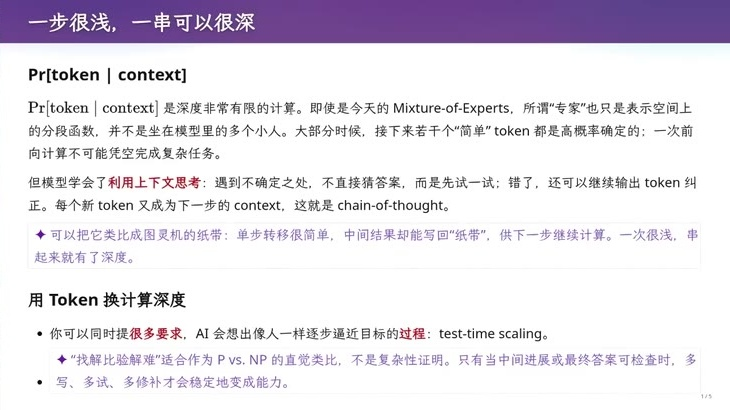
\includegraphics[width=0.94\linewidth,height=8.5cm,keepaspectratio]{notes/pce_depth.jpg}

\textbf{利用上下文和 token 延展推理}

\raggedright\footnotesize\color{muted}

画面证据：原视频
35:00--35:30，\href{https://www.bilibili.com/video/BV1CQt365EzW/?t=2100}{回看课堂片段}。草稿纸与复杂性问题仅用于建立直觉，不是计算能力的形式证明。

\end{minipage}\par\addvspace{1em}

\subsection{约束写作题把验收拆给我们看}\label{ux7ea6ux675fux5199ux4f5cux9898ux628aux9a8cux6536ux62c6ux7ed9ux6211ux4eecux770b}

课堂给出多项约束同时成立的写作任务，例如藏头、嵌字、押韵与动物故事；又讨论了相同偏旁和同音故事。这里值得观察的并不是某一首诗是否惊艳，而是模型能否逐项组织条件、发现不满足的部分并修补。

官方讲义整理了一句用于同偏旁检查的样例：``洪涝淹没江港渔浦，油污漂浮，沈涛泅渡济溺。''它去掉标点后是十八个字，都含三点水。它也暴露出规格问题：``字形中含三点水''与``字典里归为同一部首''并不必然是相同的检查规则。这是参考资料中的整理样例，不作为本地
ASR 原文引用。

\Needspace{11\baselineskip}

\begin{longtable}[]{@{}lll@{}}
\toprule\noalign{}
要求类型 & 可能的检查方式 & 检查没有覆盖的部分 \\
\midrule\noalign{}
\endhead
\bottomrule\noalign{}
\endlastfoot
藏头、字数、指定字 & 按字符顺序逐项核对 & 故事是否自然、表达是否生硬 \\
同偏旁 & 先定义判据，再查字形或字典 & 判据本身是否符合原意 \\
同音、押韵 & 明确声调和韵部标准 & 文学性、现代语感和可理解性 \\
\end{longtable}

形式条件通过，只能证明对应条件得到满足。通顺、趣味、文学性需要另外评价；代码通过几个测试，也不能自动证明需求完整、接口合理和真实场景可用。

\par\addvspace{1em}\noindent\begin{minipage}{\linewidth}\centering


\includegraphics[width=0.94\linewidth,height=8.5cm,keepaspectratio]{notes/pce_verifier.jpg}

\textbf{形式验证与质量评价的边界}

\raggedright\footnotesize\color{muted}

画面证据：原视频
45:00--45:30，\href{https://www.bilibili.com/video/BV1CQt365EzW/?t=2700}{回看课堂片段}。课堂区分检查器看得到的形式条件与没有覆盖的品味和表达质量。

\end{minipage}\par\addvspace{1em}

\section{5.
为什么规则越写越多，反而可能更难执行}\label{ux4e3aux4ec0ux4e48ux89c4ux5219ux8d8aux5199ux8d8aux591aux53cdux800cux53efux80fdux66f4ux96beux6267ux884c}

规则进入上下文后，模型有机会在相关时刻利用它。但``放进上下文''不等于``任何时候都可靠遵循''。随着历史变长、材料增多，要求之间可能竞争注意力，近期信息也可能更容易影响当前决定；具体表现取决于模型、工具和任务。

课堂讨论过给模型附加特殊口头习惯的做法：如果后来不再遵循，可以把它视为重新检查上下文状态的信号。但单次遗漏并不能证明上下文一定被截断或压缩，还需要观察实际配置与记录。它是经验性提示，不是严格的诊断工具。

另一个问题是规则进入产物。你要求``白色背景，不要半透明效果''，模型可能把这句话原样写成代码注释。于是使用者再增加一条永久规则，禁止类似注释。每遇到一个问题都追加全局要求，可能把整个上下文变成一份越来越难协调的合同。

更有效的组织方式，是区分稳定、反复适用的项目约定与当前任务细节。长期规则保持简短；任务方法按需加载；可以机械检查的条件尽量交给程序。背景颜色由样式与渲染确认，接口约束由检查或测试确认，不必无限追加自然语言劝诫。

本章小结：上下文工程也包含删减与分层。关键要求应该靠近关键决定，事实、规范与历史过程不宜混成一团。

\par\addvspace{1em}\noindent\begin{minipage}{\linewidth}\centering


\includegraphics[width=0.94\linewidth,height=8.5cm,keepaspectratio]{notes/pce_attention.jpg}

\textbf{规则副作用与按需加载}

\raggedright\footnotesize\color{muted}

画面证据：原视频
52:30--53:00，\href{https://www.bilibili.com/video/BV1CQt365EzW/?t=3150}{回看课堂片段}。否定要求可能进入产物；长期约定、任务细节和程序检查需要分层。

\end{minipage}\par\addvspace{1em}

\section{6.
``你是一位审稿人''，为什么仍然不够}\label{ux4f60ux662fux4e00ux4f4dux5ba1ux7a3fux4ebaux4e3aux4ec0ux4e48ux4ecdux7136ux4e0dux591f}

角色提示能改变语气、关注点与输出结构，却不自动提供专业判断的方法。模型很容易按``总结贡献、列出优点和不足、给出接收建议''的格式写出一份审稿意见，真正困难的是这些判断是否有依据。

论文的信息密度很高。作者已经选择问题、术语、比较对象和评价标准；如果读者只沿着文章走完一遍，很容易接受作者设定的整个框架，再在框架内部提出几条意见。看起来在批判性思考，实际上没有检验最重要的前提。

\subsection{先对齐知识边界，再评价增量}\label{ux5148ux5bf9ux9f50ux77e5ux8bc6ux8fb9ux754cux518dux8bc4ux4ef7ux589eux91cf}

课堂先让 Agent
总结一篇论文，再追问它与既有工作相比究竟新增了什么。重点不是一概不信任作者，而是先把相关领域已经解决的问题、解决程度和未解决的缺口摆出来，再判断本工作怎样向前推进。逻辑自洽、确实做完和具有值得发表的增量，并不是同一件事。

对学生读教材，这个方法可以变成知识起点的对齐：说明已经学过哪些课程、能够理解什么例子，让解释从双方共享的概念出发。只说``讲简单一点''，不如明确告诉
Agent 自己卡在何处，以及哪些基础已经掌握。

课堂还举了一个性能优化的估算例子：整体工作分为 A1 与 A2，如果 A1 大约占
99\%，A2 只占 1\%，仅说``A2 优化了
10\%''并不能说明整体获得了重要收益。按串行时间相加、其他部分不变的简化假设，编辑推导得到整体时间减少约
\(1\%\times10\%=0.1\%\)。这些比例是课堂用于检验论证意义的示例，不是某篇论文已经核实的测量数据。

这个问题提醒我们：局部实验即使正确，也仍要解释为什么值得优化这一部分。审稿不能只问``结果有没有改善''，还要问它改变了哪个重要问题、收益是否落在实际瓶颈上。

因此，与其只反复强调``严格审稿''，不如设计不同的检查路线：从主张出发，为每项贡献寻找应满足的判据；从证据出发，把实验支持、未验证假设与替代解释对应起来；从复现或反方立场出发，寻找可重算的结果、最小反例和能推翻结论的观察。

独立路线的价值来自问题不同。若所有参与者一开始就共享总体印象，最后可能只得到同一份意见的几种润色。先形成独立判断，再讨论分歧，才更有机会发现盲区。多
Agent 是组织这种工作的一个选项，数量本身不能证明独立性或正确性。

\par\addvspace{1em}\noindent\begin{minipage}{\linewidth}\centering

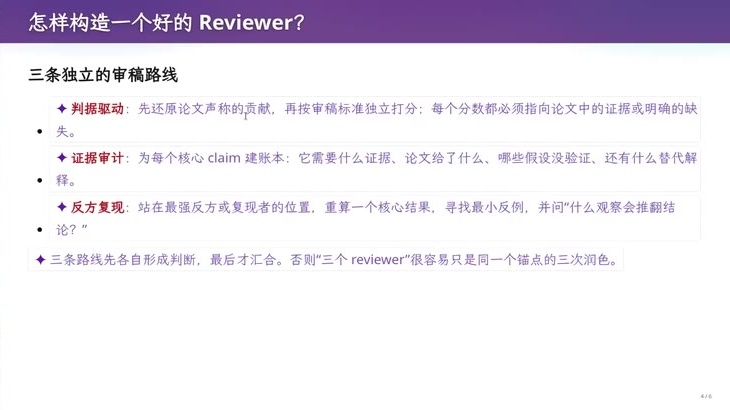
\includegraphics[width=0.94\linewidth,height=8.5cm,keepaspectratio]{notes/pce_review.jpg}

\textbf{三条独立的审稿路线}

\raggedright\footnotesize\color{muted}

画面证据：原视频
70:00--70:30，\href{https://www.bilibili.com/video/BV1CQt365EzW/?t=4200}{回看课堂片段}。课堂分别从判据、证据和反方视角安排审查，强调独立判断后再汇总。

\end{minipage}\par\addvspace{1em}

\subsection{Skill
应保存什么}\label{skill-ux5e94ux4fddux5b58ux4ec0ux4e48}

当一套方法多次有效，可以把它沉淀成
skill。值得保存的不只是``你要认真''之类的态度，而是搜索顺序、判断标准、关键检查点，以及何时需要回到证据。机械步骤交给脚本，较长资料按需引用，可以使核心方法更清楚。

Skill
也有成本。把所有可能的要求都写进去，它就变成另一道复杂的指令遵循题。复用经验要保留真正改变决策的内容，也要不断根据失败和新证据修订。

\par\addvspace{1em}\noindent\begin{minipage}{\linewidth}\centering

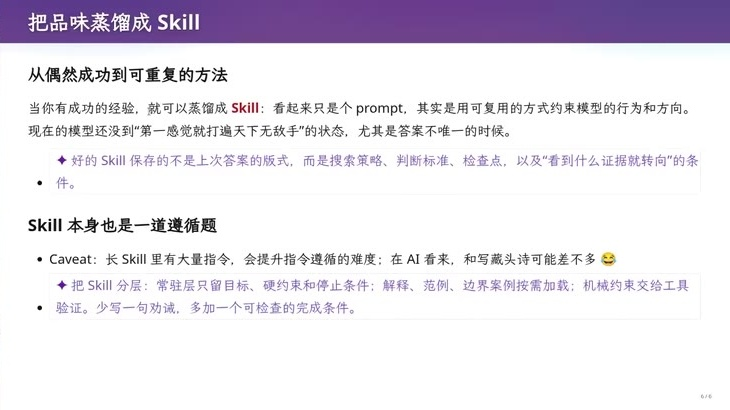
\includegraphics[width=0.94\linewidth,height=8.5cm,keepaspectratio]{notes/pce_skills.jpg}

\textbf{把成功方法沉淀为 Skill}

\raggedright\footnotesize\color{muted}

画面证据：原视频
75:00--75:30，\href{https://www.bilibili.com/video/BV1CQt365EzW/?t=4500}{回看课堂片段}。保存可复用的搜索策略和判断标准；技能本身同样有指令复杂度。

\end{minipage}\par\addvspace{1em}

\section{7.
代码库为什么本身也是上下文}\label{ux4ee3ux7801ux5e93ux4e3aux4ec0ux4e48ux672cux8eabux4e5fux662fux4e0aux4e0bux6587}

课堂提出一个观察：成熟代码库很大，Agent
却可能完成复杂修改；从零做一个似乎简单的项目，反而容易越改越乱。一个解释是，自由度与文件数量不是同一回事。成熟项目已经决定命名、分层、错误传播、测试位置与接口习惯，局部任务可以沿着附近的例子推进。

空项目没有这些约束。每次局部实现都可能顺手作出一个长期决定；若最初形成混乱惯例，后续生成又把这些惯例当作样例，问题就不断累积。因此代码库不只是待编辑的对象，也在示范``这里通常怎样做''。

这并不意味着大仓库一定好改，或者模型一定会识别最佳实践。历史包袱同样可能被模仿。课堂提出过借鉴相近领域优雅系统的设想，它应保留为待验证的方向，而不是``给模型读大项目必然提高质量''的结论。

参考的价值取决于约束是否相近、例子是否合适，以及它有没有降低后续修改成本。人的领域知识仍然重要：理解接口、不变量、状态和失败模式，才能分辨哪些结构值得沿用。

\par\addvspace{1em}\noindent\begin{minipage}{\linewidth}\centering

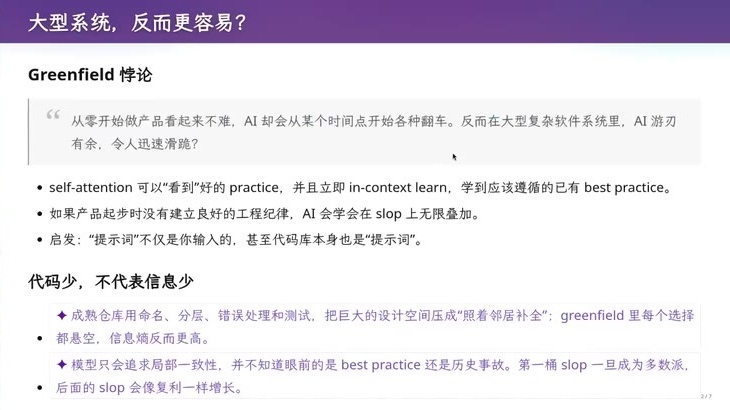
\includegraphics[width=0.94\linewidth,height=8.5cm,keepaspectratio]{notes/pce_codebase.jpg}

\textbf{代码库的上下文与自由度}

\raggedright\footnotesize\color{muted}

画面证据：原视频
77:30--78:00，\href{https://www.bilibili.com/video/BV1CQt365EzW/?t=4650}{回看课堂片段}。文件多不等于当前任务选择多；课堂把大系统与空项目作对比，结论带有适用条件。

\end{minipage}\par\addvspace{1em}

\section{8.
长程编程与长程研究缺少的是同一种反馈吗}\label{ux957fux7a0bux7f16ux7a0bux4e0eux957fux7a0bux7814ux7a76ux7f3aux5c11ux7684ux662fux540cux4e00ux79cdux53cdux9988ux5417}

构建、运行、测试、观察、修改，能为编程任务建立持续闭环。编译器报错可以指出局部问题，失败测试可以给出具体反例，Agent
于是有机会在一次失败后继续推进。长程能力依赖可利用的反馈，不只是``允许它一直运行''。

研究任务的反馈常常稀疏而含糊。课堂提到尝试优化符号执行引擎、投入很多
token
却没有得到预期结果的经历。视频里，讲师将一次关键偏差定位到``我想证明 A
方法有用''的任务表述：Agent 过于追求证明原想法，构造许多小 benchmark
寻找结论，却逐渐偏离研究真正需要回答的问题。这是讲师对该次过程的回顾，不是所有研究失败的通用归因。

例如，总 benchmark
没有变快，可能涉及求解器耗时、搜索策略、缓存收益或新增开销。这些是帮助设计下一步实验的候选解释，不是课堂已完成的归因。要让反馈更有分辨率，应先测量瓶颈，再针对某个机制建立小实验。

研究还可能把``把原想法实现好''误当成全部目标。如果假设本身不成立，更多实现并不能证明它成立。更值得问的是：什么结果会支持这个想法，什么结果会推翻它？缩小未知、排除无效方向，也可以是研究推进。

讲师回顾的纠正方向，是回到真实工具与有代表性的算法。即使完整 benchmark
跑了很久仍超时，超时前留下的搜索路径也可能揭示哪些程序结构让现有方法困难。小实验并非越小越好：它需要保留真实问题中决定成败的结构，而不是只为给原想法找一个好看的正面结果。

\par\addvspace{1em}\noindent\begin{minipage}{\linewidth}\centering

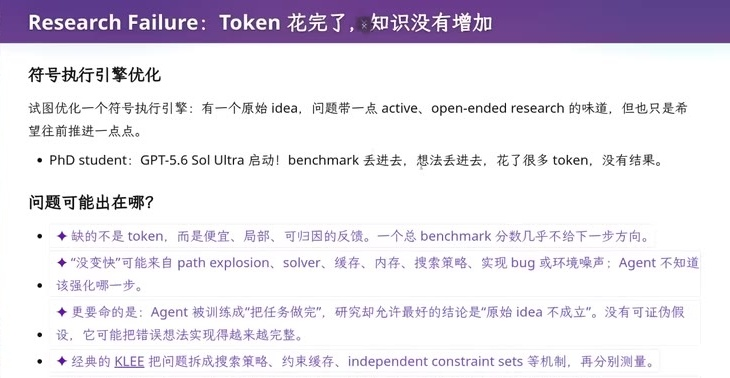
\includegraphics[width=0.94\linewidth,height=8.5cm,keepaspectratio]{notes/pce_research.jpg}

\textbf{研究失败与反馈分辨率}

\raggedright\footnotesize\color{muted}

画面证据：原视频
87:30--88:00，\href{https://www.bilibili.com/video/BV1CQt365EzW/?t=5250}{回看课堂片段}。课件列出反馈与目标方面的候选解释；视频中讲师另回顾了任务表述导致的偏向，以及回到真实工具和搜索路径的纠正。

\end{minipage}\par\addvspace{1em}

\section{9.
人应该在哪些地方投入注意力}\label{ux4ebaux5e94ux8be5ux5728ux54eaux4e9bux5730ux65b9ux6295ux5165ux6ce8ux610fux529b}

课堂提出一个取舍：你可能知道怎样让某个任务更快完成，却不一定应该时时干预。单个任务的耗时与一个人一天能够推进的事情总量，是不同的优化目标。机器多绕一点路，如果最后仍能交出可检查的结果，可能换回更重要的人类时间。

放手需要条件。接口已经讨论清楚、结果能检验、局部实现能够替换时，可以让
Agent
多探索；会扩散到多个模块的接口决定，昂贵或难恢复的动作，则值得提前关注。注意力应按影响范围和返工代价分配，而不是平均撒到每一行代码。

长任务中，日志、补丁和历史消息会不断增长。阶段切换时重新确认目标、接口和未决问题，把可检查的不变量落成测试，能让错误更早暴露。压缩上下文时应保存当前约束和证据，而不只是记录``先做了什么，后来又做了什么''。

本章小结：人的放手与验证机制应配套。反馈越清楚，重复、可恢复的尝试越容易交给机器。

\par\addvspace{1em}\noindent\begin{minipage}{\linewidth}\centering

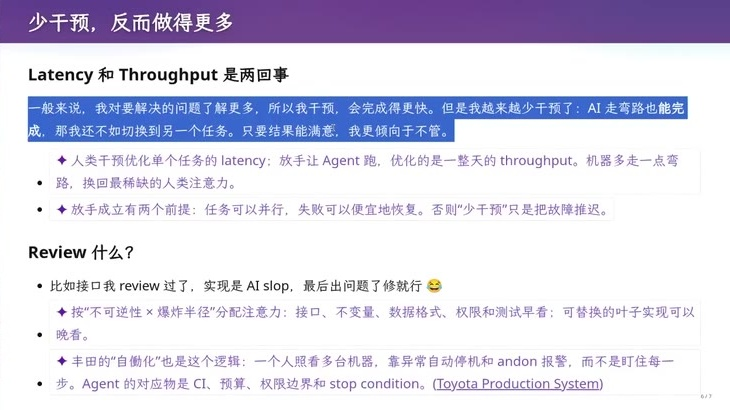
\includegraphics[width=0.94\linewidth,height=8.5cm,keepaspectratio]{notes/pce_human.jpg}

\textbf{少干预与整体吞吐量}

\raggedright\footnotesize\color{muted}

画面证据：原视频
90:00--90:30，\href{https://www.bilibili.com/video/BV1CQt365EzW/?t=5400}{回看课堂片段}。课堂区分单任务耗时与全天任务总量，并讨论应该审查哪些边界。

\end{minipage}\par\addvspace{1em}

\section{10.
怎样把更多算力变成更多有效探索}\label{ux600eux6837ux628aux66f4ux591aux7b97ux529bux53d8ux6210ux66f4ux591aux6709ux6548ux63a2ux7d22}

有些任务没有现成答案。要求``帮我想几种方案''，模型给出几个合理选项，数量要求已经满足；更有价值的方向可能仍未探索。沿同一路线继续推理，与主动寻找不同路线，是不同的计算资源使用方式。

课堂用给蒋姓小孩取名字说明这一点。直接索要几个好听、有寄托的名字，容易得到常见组合。增加数量可能仍是重复相近风格；更有用的办法是先划分典故、音韵、方言、时代感等方向，再检查出处、谐音、书写与实际偏好。

不同 Agent
可以独立提出候选或挑错，但它们是否真正探索了不同方向，比窗口数量更重要。如果共享相同前提、相同样例和同一个总体偏好，多次调用也可能高度相似。

扩大候选空间必须同时设计筛选标准。没有足够分辨率的评价，可能只是把一个平庸答案变成许多平庸答案。人需要知道什么值得留下，哪些出处应核实，什么反例足以淘汰一个方案。

课堂把这一思想联系到人与人之间的交流：每个人的经历和知识都有限，讨论的价值常常来自发现自己的默认前提。不同局限互相补充，可以扩大能够看见的问题空间。群体的收益来自差异的组织，而不是简单重复。

结尾关于算力集中与未来智力差距的描写，是讲师对未来可能性的担忧，不是已经验证的终局预测。对当前实践，更直接的启发是把资源分配给有差异的探索，并用证据筛选结果。

\par\addvspace{1em}\noindent\begin{minipage}{\linewidth}\centering


\includegraphics[width=0.94\linewidth,height=8.5cm,keepaspectratio]{notes/pce_exploration.jpg}

\textbf{用多样化候选扩大探索}

\raggedright\footnotesize\color{muted}

画面证据：原视频
95:00--95:30，\href{https://www.bilibili.com/video/BV1CQt365EzW/?t=5700}{回看课堂片段}。取名字是探索案例；先组织方向差异，再用实际偏好、出处和谐音筛选。

\end{minipage}\par\addvspace{1em}

\par\addvspace{1em}\noindent\begin{minipage}{\linewidth}\centering


\includegraphics[width=0.94\linewidth,height=8.5cm,keepaspectratio]{notes/pce_future.jpg}

\textbf{算力集中与未来可能性}

\raggedright\footnotesize\color{muted}

画面证据：原视频
97:30--98:00，\href{https://www.bilibili.com/video/BV1CQt365EzW/?t=5850}{回看课堂片段}。结尾的墙内外图像表达未来担忧，本讲义不把它当作已经验证的预测。

\end{minipage}\par\addvspace{1em}

\section{小结与练习}\label{ux5c0fux7ed3ux4e0eux7ec3ux4e60}

提示词与上下文工程的主线，是把目标、约束、样例、已有结构与反馈放到合适的位置。短程任务需要清楚的完成标准；长程任务需要可持续的反馈；开放探索则需要方向差异与筛选机制。人的方法论决定了这些资源怎样被组织。

编辑练习：选一个真实的小任务，分别写出一句模糊要求和一份带验收条件的说明。先预测两者会在哪些地方产生不同默认选择，再比较结果；挑一处失败，判断需要增加证据、修改标准、调整方法，还是建立程序检查。保留失败记录，不只保存最好看的截图。

\Needspace{12\baselineskip}

\section{来源与许可}\label{ux6765ux6e90ux4e0eux8bb8ux53ef}

\begin{itemize}
\tightlist
\item
  原课程：蒋炎岩，南京大学《生成式软件工程》2026 年第 2
  讲。\href{https://www.bilibili.com/video/BV1CQt365EzW/}{B 站回放}。
\item
  \href{https://jyywiki.cn/GSE/2026/lect2.md}{官方讲义《提示词与上下文工程》}与\href{https://jyywiki.cn/GSE/2026/slides2.html}{课堂课件}。
\item
  本文为课程重组与解释，保留讲师观点、未验证设想与编辑补充之间的区分。相关课程改编内容按
  \href{https://creativecommons.org/licenses/by-nc/4.0/}{CC BY-NC 4.0}
  署名、非商业使用与许可条件提供，不代表讲师或学校认可。
\end{itemize}

核验材料见仓库
\texttt{evidence/nju-gse-02/}，包括完整音轨的窗口转录、媒体哈希、所选画面出处、时间段覆盖表及检查范围。未作逐字听写、逐帧全检或全部课堂演示复现。

\end{document}
